\documentclass{llncs}
\usepackage[ruled,vlined,linesnumbered]{algorithm2e}
\usepackage{color,graphicx,epstopdf,changepage,amsmath,multirow}
\usepackage[justification=centering]{caption}
\SetAlgoCaptionSeparator{.\space}
\renewcommand\AlCapFnt{\normalfont\scshape}
\setlength{\algomargin}{0.7cm}

\title{Comprehensive Quality Awareness Automated Semantic Web Service Composition}
\author{Chen Wang, Hui Ma, Aaron Chen and Sven Hartmann}
\institute{School of Engineering and Computer Science,
\\Victoria University of Wellington, New Zealand \\
Email: \{chen.wang, hui.ma, aaron.chen\}@ecs.vuw.ac.nz}

\usepackage[pdfauthor={\@author}, pdftitle={\@title}]{hyperref}
\makeatother

%\providecommand{\e}[1]{\ensuremath{\times 10^{#1}}}
\vspace{-1.5cm}

\begin{document}
\maketitle
\begin{abstract}
Semantic web service composition has been a prevailing research area in recent years. There are two major challenges faced by researchers, semantic matchmaking and Quality of Service (QoS) optimisation. Semantic matchmaking aims to discover interoperable web services that can interact with each other by their resources described semantically. QoS optimisation aims to optimise the non-functional requirements of service users, e.g., minimum cost, maximal reliability. To meet users' requirements, one often needs to consider both semantic matchmaking quality and QoS simultaneously. Existing works on web service composition focus mainly on one single type of requirements. Therefore, we propose a comprehensive quality model considering semantic matchmaking quality and QoS simultaneously with an aim of achieving a more desirable balance on both sides. Further more, we develop a PSO-based service composition approach with explicit support for the comprehensive model. We also conduct experiments to address the effectiveness of our PSO-based approach and a desirable balance achieved using our comprehensive quality model.

%where PSO optimise a queue of task-related services that is decoded into composition solutions. We compare the effectiveness of PSO-based method with one recent GP-based method using the proposed comprehensive quality model, and also compare the effectiveness of our proposed comprehensive quality model with one promising QoS model.

\end{abstract}
\section{Introduction}\label{introduction}

\textit{Web service composition} pertains to a chain of multiple web services to provide a value-added composite service that accommodates customers' complex requirements. 
%This application is developed by integrating interoperable and collaborative functionalities over heterogeneous systems. 

Two most notable challenges for web service composition are ensuring interoperability of services and achieving Quality of Service (QoS) optimisation \cite{fensel2011semantic}. \textit{Interoperability} of web services presents challenge in syntactic and semantic dimensions. The syntactic dimension is covered by the XML-based technologies, such as $WSDL$, $SOAP$. The semantic dimension enables a better collaboration through ontology-based semantics, such as OWL-S, WSML, and SAWSDL \cite{petrie2016web}. \textit{Semantic web services composition} is distinguished from the syntactic service composition, the resources of semantic web services are described semantically to enable a better interoperability for chaining web services. The second challenge is related to QoS optimisation. This problem gives birth to \textit{QoS-aware service composition} that aims to find composition solutions with optimised QoS.

Existing works on service composition focus mainly on addressing only one challenge above. In these works, huge efforts have been devoted to QoS-aware web service compositions assuming a pre-defined abstract workflow is given. This is generally considered as a \textit{semi-automated web service composition} approach \cite{parejo2008qos}. Generating composition plans automatically in discovering and selecting suitable web services is a NP-hard problem \cite{moghaddam2014service}. In the past few years, many approaches \cite{gupta2015optimization,ma2015hybrid,qi2010combining,da2016particle,da2015graphevol,yu2013adaptive} to QoS-aware web service composition employ Evolutionary Computation (EC) techniques to automatically generate composition solutions, but few works have enabled an \textit{automatic semantic web service composition}, where both QoS and quality of semantic matchmaking are optimised simultaneously to achieve a desirable balance on both sides.  

The overall goal of this paper is to \textit{develop a PSO-based approach to automated comprehensive quality-aware semantic web service composition that satisfactorily optimises both QoS and semantic matchmaking quality}. Particularly, this paper extends existing works of QoS-aware service composition by considering jointly optimising QoS and semantic matchmaking quality using our proposed comprehensive quality model. Particle Swarm Optimisation (PSO) has shown promise in searching for near-optimised service composition solutions \cite{da2016particle}. We will propose a PSO-based service composition approach with explicit support for our proposed quality model. We will achieve three objectives in this work:

\begin{enumerate}
 \item To propose a comprehensive quality model that addresses QoS and semantic matchmaking quality simultaneously with a desirable balance on both sides.
  
 \item To propose a PSO-based service composition approach using the proposed comprehensive quality model. To do that, we aim to find a service candidate queue that can be decoded into a service composition with the near-optimal comprehensive quality.  
 \item To address the effectiveness of our PSO-based approach and a desirable balance achieved using our comprehensive quality model, we first compare our PSO-based approach with one recent GP-based approach \cite{ma2015hybrid} using our proposed quality model, and then compare our proposed quality model with one widely used QoS model using our proposed PSO-based approach.
\end{enumerate}
\section{Related Work} \label{relatedWork}
Substantial works on web service composition focus on either semantic web service composition \cite{bansal2016generalized,boustil2014semantic,mier2015integrated} or QoS-aware web service composition \cite{gupta2015optimization,ma2015hybrid,qi2010combining,da2016particle,da2015graphevol,yu2013adaptive}, However, only a few researchers address both semantic matchmaking quality and QoS for web service composition problems. To the best of our knowledge, \cite{fanjiang2014semantic,lecue2009optimizing,pop2009immune} reported some attempts on service composition that considers both aspects.

Semantic web service composition \cite{bansal2016generalized,boustil2014semantic,mier2015integrated} captures the semantic descriptions of web services' parameters using some kind of logic (e.g., description logic) that ensuring the interoperability of web services. In these approach, the number of web services or length of a graph representation for web service composition is minimised to reach the optimised composition solutions. However, this evaluation approach does not guarantee an optimised QoS of composition solutions.

QoS-aware web service composition is studied using traditional approaches or Evolutionary Computation (EC) techniques for finding near-optimised solutions. Qi et al. \cite{qi2010combining} propose a local optimisation and enumeration method, where a small number of promising candidates related to each task are considered by local selection, and composition solutions are enumerated to reach the near optimal QoS. EC techniques are widely used to automatically generate solutions with optimal QoS. Gupta et al. \cite{gupta2015optimization} employ a modified Genetic Algorithm (GA) using a binary string as an individual, which demands to be decoded into composition solutions. Yu et al.  \cite{yu2013adaptive} use Genetic Programming (GP) for finding optimal solutions that are reached by penalising infeasible solutions using a fitness function. A hybrid approach employing a greedy search and GP is introduced in \cite{ma2015hybrid} to generate functionally correct tree-based individuals, which are transformed from \emph{directed acyclic graph}s (DAGs). To eliminating the transformation process, a promising GraphEvol is proposed in \cite{da2015graphevol}, where graph-based evolutionary operators are employed. An indirect PSO-based approach was introduced in \cite{da2016particle}. An service queue is used as an indirect representation that is decoded into a DAG. These QoS-aware approaches \cite{gupta2015optimization,qi2010combining,ma2015hybrid,da2016particle,da2015graphevol,yu2013adaptive} do not consider semantic matchmaking quality.

Only a few works \cite{fanjiang2014semantic,lecue2009optimizing,pop2009immune} consider both semantic matchmaking quality and QoS simultaneously. Lecue et al. \cite{lecue2009optimizing} propose a semi-automated web service composition using GA to encode a given abstract service workflow, where the evaluation of semantic matchmaking quality requires a complete and formal definition of ontology using description logic that associated to the resources of web services. Another GA-based approach \cite{fanjiang2014semantic} utilise process description language to encode pre-stored cases-based workflows, where workable services are composed to complete this workflow. An automated immune-inspired web service composition approach \cite{pop2009immune} employs a clonal selection algorithm to proliferate decoded planning graphs, but this approach is only studied in some cases.

In summary, despite a large number of approaches for semantic web service composition and QoS-aware service composition approaches, there is a lack of a fully automated semantic service composition approach to optimise semantic matchmaking quality and QoS simultaneously. 
%Therefore, we first propose an automated comprehensive quality-aware semantic web service composition approach. To do that, we will design a comprehensive quality model that considers both QoS and quality of semantic matchmaking between services. We will then propose a PSO-based approach to this semantic service composition using our proposed comprehensive quality model to evaluate candidate solutions.  

\section{Motivation and Problem Description}\label{Motivation and Problem Description}\label{Motivation}\label{problemDes}\label{qualityModel}\label{Comprehensive_Quality_Model}\label{qualityModel}

Our goal is to develop a PSO-based approach for automatically generating good service compositions. Often, many different service compositions can meet a user request but differ significantly in terms of QoS and semantic matchmaking quality. For example, in the classical travel planning context, some component service must be employed to obtain a travel map. Suppose that two services can be considered for this purpose. One service $S$ can provide a street map at a price of 6.72. The other service $S'$ can provide a tourist map at a price of 16.87. Because in our context a tourist map is more desirable than a street map, $S'$ clearly enjoys better semantic matchmaking quality than $S$ but will have negative impact on the QoS of the service composition (i.e., the price is much higher). One can easily imagine that similar challenges frequently occur when looking for service compositions. Hence, a good balance between QoS and semantic matchmaking quality is called for. We therefore propose a comprehensive quality model in considering semantic matchmaking quality and QoS simultaneously.

We consider a \emph{semantic web service} (\emph{service}, for short) as a tuple $S = (I_{S}, O_{S}, QoS_S)$ where $I_{S}$ is the set of service inputs that are consumed by $S$, $O_{S}$ the set of service outputs that are produced by $S$, and $QoS_{S}=\{t_S, c_S, r_S, a_S\}$ the set of non-functional attributes of $S$. The inputs in $I_{S}$ and the outputs in $O_{S}$ are concept-related parameters with the concepts in an ontology $\mathcal{O}$. The attributes $t_S, c_S, r_S, a_S$ refer to the response time, cost, reliability, and availability of service $S$, respectively. These four QoS attributes are most commonly used \cite{zeng2003quality}.
% \textit{Response time} ($t_S$) measures the expected delay in seconds between the moment when a request is sent and the moment when the results are received. \textit{Cost} ($c_S$) is the amount of money that a service requester has to pay for executing the service. \textit{Reliability} ($r_S$) is the probability that a request is correctly responded within the maximum expected time frame, which is expressed as a number between 1 and 0. Similarly, \textit{availability} ($a_S$) is the probability that a service is accessible. 

A \emph{service repository} $\mathcal{SR}$ is a finite collection of services with a common ontology $\mathcal{O}$. A \emph{service request} (also called \emph{composition task}) over $\mathcal{SR}$ is a tuple $T=(I_{T}, O_{T})$ where $I_{T}$ is the set of task inputs, and $O_{T}$ the set of task outputs. The inputs in $I_{T}$ and the outputs in $O_{T}$ are concept-related parameters with the concepts in the ontology $\mathcal{O}$.

A service composition is commonly represented as a DAG. It nodes correspond to the services in the composition. Two services $S$ and $S'$ are connected by an edge $e$ if some output of $S$ serves as input for $S'$. Apparently, such outputs and inputs must semantically match to ensure the correct execution of the service composition. 
%Moreover, the overall service inputs and outputs associated with the DAG must satisfy the composition requirements provided by users.
%To answer a request from a user a suitable service composition is sought. 
The mechanism to compose services relies on the semantic descriptions of inputs and outputs, which enables inputs of services to be matched by outputs of other services. The following \emph{matchmaking types} are often used to describe the level of a match \cite{paolucci2002semantic}: For concepts $a, b$ in $\mathcal{O}$ the \emph{matchmaking} returns $exact$ if $a$ and $b$ are equivalent ($a \equiv b$), $plugin$ if $a$ is a sub-concept of $b$ ($a \sqsubseteq b$), $subsume$ if $a$ is a super-concept of $b$ ($a \sqsupseteq b$), and $fail$ if none of previous matchmaking types is returned.
%($a \perp b$)
In this paper we are only interested in robust compositions where only $exact$ and $plugin$ matches are considered, see \cite{lecue2009optimizing}. 
%
As argued in \cite{lecue2009optimizing} $plugin$ matches are less preferable than $exact$ matches due to the overheads associated with data processing. We suggest to consider the semantic similarity of concepts when comparing different plugin types. For concepts $a, b$ in $\mathcal{O}$ the \emph{semantic similarity} $sim(a, b)$ is calculated based on the edge counting method defined in the formula (\ref{equation1}) from \cite{shet2012new}, where $N_a$, $N_b$ and $N_c$ measure the distances from concept $a$, concept $b$, and a closest common ancestor $c$ of $a$ and $b$ to the top concept of the ontology $\mathcal{O}$, respectively. 

\begin{equation}
sim(a, b){=} \frac{2N_c \cdot e^{-\lambda L/D} }{N_{a}+N_{b}}
\label{equation1}
\end{equation}

\noindent For our purposes, $\lambda$ can be set to 0 as we do not measure the similarities of neighbourhood concepts, which is not the matching type considered in this paper. 
%Thus, we obtain a combined function for measuring semantic matchmaking quality between two concepts:

%\begin{equation}\label{equation2}sm(a, b) \stackrel{.}{=} ( type(a, b), \  sim(a, b) )\end{equation}

Given a service request $T=(I_T,O_T)$, we represent a service composition solution for $T$ with services $S_1,\ldots,S_n$  by a weighted DAG, $WG=(V,E)$ with node set $V=\{Start, S_1, S_2, \ldots, S_n, End\}$ and edge set $E = \{e_{1}, e_{2},... e_{m} \}$. $Start$ and $End$ are two special services defined as $Start = (\emptyset, I_T, \emptyset )$ and $End  = (O_T, \emptyset, \emptyset)$ that account for the input and output requirements given by the request. 
%Each edge $e$ between two services $S$ and $S'$ is associated with a set of incoming outputs produced by $S$ and a set of outgoing inputs consumed by $S'$.
Each edge $e$ from a service $S$ to a service $S'$ means that service $S$ produces an output $a\in O_S$ that is matched ($exact$ or $plugin$) to an input $b\in I_{S'}$ to be consumed by service $S'$ in the composition. Based on the matchmaking type the \emph{semantic matchmaking quality} of edge $e$ can be defined as follows:

\begin{equation}
\label{equation10}
type_e = 
\begin{cases}
	1 & \text{ if $a\equiv b$ ($exact$ match)},\\
	p & \text{ if $a \sqsubseteq b$ ($plugin$ match)}
\end{cases}
\end{equation}
\begin{equation}
\label{equation11}
sim_e = sim(a,b) = \frac{2N_c}{N_{a}+N_{b}}
\end{equation}

\noindent with a suitable parameter $p, 0<p< 1$ to chosen, for discussion see Section \ref{PSO_based_approach}. However, if more than one pair of matched output and input from services $S$ and $S'$ respectively, $type_e$ and $sim_e$ will take on their average values.

%$e = \{ (O_{S_{src}} \cup I_{S_{src}}) \mid \forall o \in O_{S_{src}}, \exists i \in O_{S_{src}} \wedge fullmatch (o \Rightarrow i) \}$

%\textbf{Definition 4.} Given $(a \in O^{C}_{S_m}) \vee (b \in I^{C}_{S_n}) \wedge (m \neq n) $, a $full match(a \Rightarrow b)$ holds if $type(a, b)$ returns $exact$ or $plugin$. The operator ``$ \Rightarrow$'' means $a$ is passed to $b$, and $b$ is fully satisfied by $a$. The full match is a guarantee of completely valid  ``$ \Rightarrow$'' operation, whereas, partial matches are not considered in this paper.

%\textbf{Semantic matchmaking quality model}. Due to that the discretisational characteristics of different match types and values assigned to matching types driven by the cost of data manipulation \cite{lecue2009optimizing}, match types are considered to be one factor for the quality of matchmaking. For example, Exact matching type demands less time for computation compared to that of Plugin match. Another factor is concept similarity of two matched concepts. For example, two plugin types, $publication \sqsubseteq printedmaterial$ and $romanticnovel \sqsubseteq printedmaterial$, are associated with different similarities.

%\textbf{Definition 5.} Given $full match(a \Rightarrow b)$, $sim(a, b)$ is a function that given a output-related concept $a$ of a service and a input-related concept $b$ of another service, it returns a concept similarity value between $a$ and $b$.

%\textbf{Definition 6.} Given $full match(a \Rightarrow b)$, $sm(a,b)$ is a function for measuring semantic matchmaking quality between two concepts, which returns a pair of values consisting of $type(a, b)$ and $q_{sim}(a, b)$ defined in Formula (\ref{equation2}).

%\textbf{Weighted DAG composition model}. web service composition is considered to be a data workflow, where services are chained together by their inputs and outputs using the two models defined before. All these concepts are captured and tackled in a weighted DAG as $WG = (V, E)$ , where:

%\textbf{Comprehensive quality model in a weighted DAG}. 

%Since each $e$ defined in $E$ could have more than one $fullmatch(a \Rightarrow b)$ form a edge. Therefore, semantic matchmaking quality of one edge, denoted as $sm_e$ is defined in formula (\ref{equation3}), where $type_{e}$ and $sim_{e}$ are the average values of all involved $type(a, b)$ and $q_{sim}(a, b)$ respectively. 

%\begin{equation}\label{equation3}sm_{e} \stackrel{.}{=} (type_ {e}, \  sim_ {e})\end{equation}

The \emph{semantic matchmaking quality} of the service composition can be obtained by aggregating over all edges in $E$ as follows:

%\begin{equation}
%\label{eqSM}
%SM \stackrel{.}{=} (MT, SIM)
%\end{equation}
\begin{equation}
\label{equation6}
MT {=} \prod_{j=1}^{m} type_ {e_{j}}
\end{equation}
\begin{equation}
\label{equation7}
SIM {=} \frac{1}{m}\sum_{j=1}^m sim_ {e_{j}}
\end{equation}
%\begin{equation}
%\label{eqCQ}
%CQ \stackrel{.}{=} (MT, \  SIM, \  A,\  R,\  C,\  T)
%\end{equation}

The \emph{QoS} of the service composition can be obtained by aggregating the QoS values of the participating services. For a service composition with services $ S_1, S_2, ... S_n$ we obtain the reliabilitiy $R=\prod\limits^n_{k=1}r_{S_k}$, the availability $A=\prod\limits^n_{k=1}a_{S_k}$, the cost $C=\sum\limits^n_{k=1}c_{S_k}$, and the response time $T$ is the time of most time-consumption path in the composition, i.e., $$T = MAX \{\sum\limits^{\ell_j}_{k=1}t_{S_k} | \text{ $j\in\{1,\ldots,m\}$ and $P_j$ is a path of length $\ell_j$}\}.$$

%Consequently, in Formula \ref{eqCQ}, the comprehensive quality $CQ$ consists of the aggregated semantic matchmaking quality $SM$ and the QoS calculation in DAG discussed before.

\noindent When multiple quality criteria are involved into decision making, then the overall fitness of a solution is evaluated by a proposed comprehensive quality model, which can be defined as a weighted sum of the individual criteria: 

\begin{equation}
\label{equation8}
Fitness = w_1 \hat{MT} + w_2 \hat{SIM} + w_3 \hat{A} + w_4 \hat{R} + w_5(1 - \hat{T}) + w_6(1 - \hat{C})
\end{equation}
\noindent with $\sum_{k=1}^{6} w_k= 1$. The weights can be adjusted according to users' preferences. Herein, the individual criteria are normalised to a range between 0 to 1, where 1 means the best value and 0 means the worst. For this purpose, we normalise $MT$, $SIM$, $A$, $R$, $T$, and $C$ so that the function value falls within the range from 0 to 1 using formula (\ref{equation9}). To simplify the presentation we also use the notation $(Q_1,Q_2,Q_3,Q_4,Q_5,Q_6) = (MT,SIM,A,R,T,C)$. $MT$ and $S$ have minimum value 0 and maximum value 1. The minimum and maximum value of $A$, $R$, $T$, and $C$ are calculated across all task-related candidates in the service repository $\mathcal{SR}$ using greedy search, for discussion see Section \ref{PSO_based_approach}.

\begin{equation}
\label{equation9}
\hat{Q_k} = 
\begin{cases}
	\frac{Q_k - Q_{k, min}}{Q_{k, max} - Q_{k, min}} & \text{ if $k=1,\ldots,4$ and }Q_{k, max} - Q_{k, min} \neq 0,\\
	\frac{Q_{k,max} - Q_k}{Q_{k, max} - Q_{k, min}} & \text{ if $k=5,6$ and }Q_{k, max} - Q_{k, min} \neq 0,\\
	1 & \text{ otherwise}.
\end{cases}
\end{equation}

\noindent The composition task is to find the maximum value of objective function in (\ref{equation8}).

%If the weights for $MT$ and $S$ are put to 0 we obtain the QoS-aware service composition approach \cite{ma2015hybrid,da2016particle,da2015graphevol} as a special case. To adequatley reflect the relevance of semantic quality it is recommended to choose he weights for $MT$ and $S$ strictly larger than 0.

\section{PSO-based Approach to Comprehensive Quality-Aware Automated Semantic Web Service Composition}\label{qswsc_approach}
\vspace{-0.8cm}
\begin{figure}[h]
\centering
\fbox{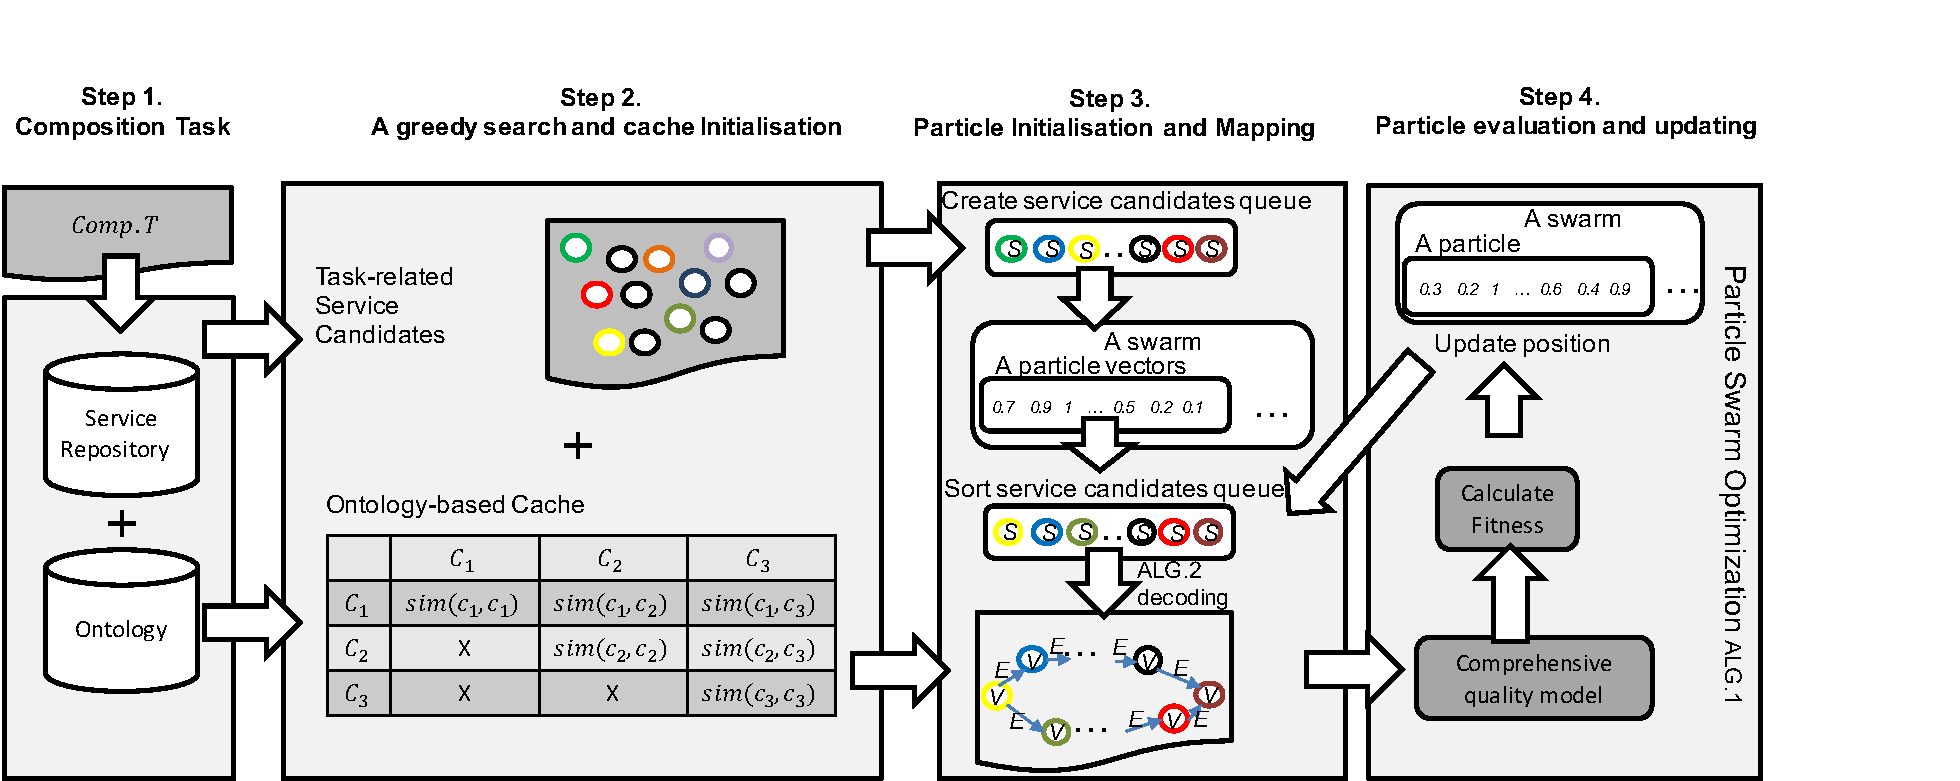
\includegraphics[scale=.4]{overview.pdf}}
 \caption{An overview of POS-based approach to comprehensive quality-aware automated semantic web service composition.}
 \label{overview}
\end{figure}
\vspace{-1.0cm}
\subsection{An Overview to PSO-based Method}\label{PSO_based_approach}

PSO has shown promise in solving combinatorial optimisation problems, and is also considered to be an easy way to maintain the correctness of solutions. For example, GP-based approaches often require repairing the solutions \cite{da2016particle}. Therefore, we employ a PSO-based approach to comprehensive quality-aware automated semantic web service composition. Fig. \ref{overview} shows an overview of our approach consisting of four steps: 

Step 1: The composition process is triggered by a composition task, which is clearly defined in \ref{problemDes}. 

Step 2: This composition task is used to discover all task-related service candidates using a greedy search algorithm adopted from \cite{ma2015hybrid}, which contributes to a shrunken service repository. This greedy search algorithm keeps adding outputs of the invoked services as available outputs (initialised with $I_{T}$) , and these available outputs are used to discover task-related services from a service repository and updated with the outputs of these discovered services. This operation is repeated until no service is satisfied by the available outputs. During the greedy search, an ontology-based cache ($cache$) is initialised that stores the concept similarities of matched inputs and outputs of task-related candidates. This $cache$ is also used to discover services by checking whether $null$ is returned by given two output-related and input-related concepts.

Step 3 and Step 4: These two steps follow the standard PSO steps \cite{shi2001particle} except for some differences in particles mapping and decoding processes. In particular, these two differences are related to sorting a created service queue using serivce-to-index mapping for a particle' position vectors and evaluating the fitness of a particle after decoding this service queue into a $WG$ respectively. Those differences are further addressed in Algorithms \ref{novelSteps} and \ref{graph_building} in \ref{POS-based_algomargin}.

\subsection{PSO-based approach algorithm}\label{POS-based_algomargin}
The overall algorithm investigated here is made up of a PSO-based web service composition algorithm \ref{novelSteps} and a decoding algorithm \ref{graph_building}. In Algorithm \ref{novelSteps}, the  steps $4$, $5$, $6$ and $7$ are different from those of standard PSO: In step 4, the size of task-related service candidates generated by a greedy search determines the size of each particle's position, and each candidate in a created service candidates queue is mapped to an index of a particle’s position vectors, where each vector has a weight value between 0.0 and 1.0. In step 5, service candidates in the queue are sorted according to their corresponding weight values in descending order. In step 6, this sorted queue is used as one of the inputs of the forward decoding algorithm \ref{graph_building} to create a $WG$. In step 7, the fitness value of this $WG$ is the fitness value of the particle calculated by the comprehensive model discussed in \ref{Comprehensive_Quality_Model}.
\begin{algorithm}
 %\LinesNumbered
 \SetKwInOut{Input}{Input}\SetKwInOut{Output}{Output}
 \SetKwFunction{generateWeightedGraph}{generateWeightedGraph}
 \SetKwProg{Procedure}{Procedure}{}{}
 \SetNlSty{}{}{:}
 Randomly initialise each particle in the swarm\;
  \While {max. iterations not met}{
     \ForEach{particles in the swarm}{
     Create a service candidates queue and map service candidates to a particle's position vectors\;
     Sort the service queue by position vectors' weights\;
     Create a weighted DAG from the service queue ( Algorithm\ref{graph_building}) \;
     Calculate the weighted DAG fitness value\;
     
      \eIf{fitness value better than pBest}{    
        Assign current fitness as new \emph{pBest}\;
       }{
        Keep previous \emph{pBest}\;
       }	
     }
    Assign best particle's \emph{pBest} value to \emph{gBest}, if better than \emph{gBest}\;
 	Calculate the velocity of each particle\;
  	Update the position of each particle\;
  }
\caption{Steps of PSO-based service composition technique \cite{da2016particle}.}
\label{novelSteps}
\end{algorithm} 


Algorithm  \ref{graph_building} is a forward graph building algorithm based on \cite{blum1997fast}. This algorithm take one input, a sorted service queue from step 5 of Algorithm \ref{novelSteps}. If service queues are sorted resulting in different service order, it is possible to create different corresponding $WGs$ as composition solutions. In addition. $I_{T}$, $O_{T}$ and $cache$ are also taken as the inputs. Firstly, $Start$ and $End$ are added to $V$ of $WG$ as an initialisation, and $OutputSet$ is also created with $I_{T}$.  If all the inputs $I_{S}$ of the first popped  $S$ from $queue$ can be satisfied by provided outputs from $OutputSet$. This $S$ is added to $V$ and its outputs are added to $OutputSet$, and $S$ is removed from $queue$. Meanwhile, $e$ is created with $type_e$ and $sim_e$ calculated. These steps are repeated until $O_{T}$ can be satisfied by $Outputset$ or the service queue is $null$. Consequently, this forward graph building technique could lead to more services and edges connected to the $WG$, which should be removed before $WG$ is returned.

\begin{algorithm}
 \SetKwInOut{Input}{Input}\SetKwInOut{Output}{Output}
 \SetKwFunction{createWeightedDAG}{createWeightedDAG}
 \SetKwProg{Procedure}{Procedure}{}{}
 %\LinesNumbered
 \SetNlSty{}{}{:}
 % \Procedure{}{
 \Input{ $I_T$, $O_T$, $queue$, $cache$}
 \Output{WG}
 $WG = (V, E)$\;
 $V \leftarrow$ \{$Start$, $End$ \} \;
 $OutputSet \leftarrow$ \{$I_{T}$\}\;
  \While { $O_{T}$ do not satisfied by $OutputSet$}{
     \ForEach{$S$ in $queue$}{
      \uIf{all $I_{S}$ satisfied by $OutputSet$}{    
        $e \leftarrow$ calcuate $type_e$, $sim_e$\;
        $E$ add $e$\;
        $V$ add $S$\;
        $OutputSet$ add \{$O_{S}$\}\;    
        $queue$.remove $S$\;
       }	
     }
  }
 remove $dangling nodes$\; 
 remove $dangling edges$\;
 \KwRet $WG$\;
 %}
 \caption{Create a weighted DAG from a  sorted queue.}
\label{graph_building}
\end{algorithm} 

\vspace{-1.0cm}

\section{Experiment Study}\label{experiment_design}
In this section, a quantitative evaluation approach is adopted in our experiment using a benchmark dataset, an augmented version of Web service challenge 2009 including QoS attributes, which is used in \cite{ma2015hybrid,da2016genetic}. Two objectives of this evaluation are to: $(1)$ measure the effectiveness of our PSO-based approach. 
%To do this, we compare our PSO-based method with one existing GP-based approach \cite{ma2015hybrid}. 
$(2)$ measure the effectiveness of our proposed comprehensive quality model for achieving desirable balance of semantic matchmaking quality and QoS. 
%To do this, we compare a widely used QoS model in QoS-aware web service composition \cite{ma2015hybrid,da2016particle,da2015graphevol} with our comprehensive quality model using our PSO-based approach.


%WSC09 is a benchmark dataset consisting of five composition tasks. These tasks are associated with an increasing number of services, and concepts in ontologies. 

The parameters are chosen based on the settings from \cite{shi2001particle} for our PSO-based approach, In particular, PSO population size is 30 with 100 generations. We run 30 times independently for each dataset. We configure the weights of fitness function to properly balance functional side and nonfunctional side. Therefore, $w_{1}$ and $w_{2}$ are set equally to 0.25, and $w_{3}$, $w_{4}$, $w_{5}$, $w_{6}$ are all set to 0.125. The returned value of $type(a,b)$ is set to 1 ($Exact$) and 0.75 ($Plugin$) according to \cite{lecue2009optimizing}. In general, weight settings and parameter match type quality are decided by users' preferences.

\subsection{Comparison Test for GP-based approach and PSO-based approach}\label{comparisonTestWithGP}
To evaluate the effectiveness of our proposed PSO-based approach, we compare one recent GP-based approach \cite{ma2015hybrid} with our PSO-based method. The semantic matchmaking quality of this GP-based approach is easy to evaluated considering measuring links between parent nodes and children nodes. Therefore, we evaluate both semantic matchmaking quality and QoS simultaneously for that GP-based approach using the proposed comprehensive quality model. To make a fair comparison, we consider the same number of evaluations (3000 times) used in our PSO-based approach. We set the parameters' settings of that GP-based approach as 30 individuals and 100 generations, it is considered to be proper settings refering to \cite{da2015gp}.

The first column of Table \ref{meanFitness} shows five tasks from WSC09 Dataset. The second and third column of Table \ref{meanFitness} show the orginal service repository size before the greedy search and shrunk service repository size after the greedy search respectively regarding the five tasks. This greedy search helps reducing the repository size by considering only task-related service candidates, which also contributes to a significant reduced researching space. The fourth and fifth column of Table \ref{meanFitness} show the mean fitness values of 30 independent runs accomplished by two methods. We employ independent-samples T tests to test the significant differences in mean fitness value. The results show that the PSO-based approach outperformes the existing GP-based approach in most cases except task 3 (all the p-values are consistently smaller than 0.01). In task 5, the PSO-based approach performs significantly better than the GP-based approach in finding optimal solutions. It may be that the GP-based approach is stuck in local optima due to the very large search space in Task 5. On the other hand, the decoding process used by the PSO-based approach allows for small changes that more effectively prevent this from happening.
\begin{table}[]
\centering
\caption{Mean fitness results for comparing GP-based approach}
\label{meanFitness}
\begin{tabular}{c|c|c|l|l}
\hline
\multicolumn{1}{c|}{WSC09} &Original $SR$  &Shrunken $SR$   &PSO-based approach & GP-based approach  \\ \hline
Task 1                     &572            &80    &0.5592 $\pm$ 0.0128  $\uparrow$  &0.5207 $\pm$ 0.0208           \\ \hline
Task 2                     &4129           &140   &0.4701 $\pm$ 0.0011  $\uparrow$  &0.4597 $\pm$ 0.0029          \\ \hline
Task 3                     &8138           &153   &0.5504 $\pm$ 0.0128              &0.5679 $\pm$ 0.0234 $\uparrow$   \\ \hline
Task 4                     &8301           &330   &0.4690 $\pm$ 0.0017  $\uparrow$  &0.4317 $\pm$ 0.0097            \\ \hline
Task 5                     &15211          &237   &0.4694 $\pm$ 0.0008  $\uparrow$  &0.2452 $\pm$ 0.0369            \\ \hline
\end{tabular}
\end{table}



\subsection{Comparison Test for Comprehensive Quality Evaluation Model and QoS Evaluation Model}\label{comparisonTest}

Recently, a QoS Evaluation Model, $Fitness = w_1 \hat{A} + w_2 \hat{R} + w_3(1 - \hat{T}) + w_4(1 - \hat{C})$, where $\sum_{i=1}^{4} w_i = 1$, is widely used for QoS-aware web service composition \cite{ma2015hybrid,da2016particle,da2015graphevol}. This QoS evluation model is compared to our proposed comprehensive quality evluation model using our proposed PSO-based approach for measuring the effectiveness of our proposed comprehensive quality model. To analyse the differences in optimal solutions found by these two evaluation models, we recorded and compared the different mean values of $SM$ (consisiting of $MT$ and $S$), $QoS$(consisting of $A$, $R$, $T$ and $C$) after 100 generations. To make a sense of the comparison, all these recorded values are normalised from 0 to 1, and compared using independent-samples T tests in Table \ref{decisionTable}. 

We observe an interesting pattern from Table \ref{decisionTable}. The mean values of $QoS$ using QoS evaluation model are significantly higher than those using comprehensive quality evaluation model for Tasks 2, 3, 4 and 5. However, the mean value of $SM$ using the comprehensive quality evaluation model are significantly higher than those using the QoS evaluation model, while a slight trade-off in $QoS$ are observed in all tasks.

\begin{table}[]
\footnotesize
\centering
\caption{Mean values of $SM$ and $QoS$ for QoS evaluation model and comprehensive quality evaluation model using PSO-based approach}
\label{decisionTable}
\begin{tabular}{c|l|l|l}
\hline
\multicolumn{2}{c|}{WSC09}              & \shortstack{QoS \\ Evaluation Model}         &\shortstack{Comprehensive Quality \\ Evaluation Model} \\ \hline
\multirow{2}{*}{Task1}  &$SM$   &0.5373 $\pm$ 0.0267               &0.5580 $\pm$ 0.0094 $\uparrow$ \\ \cline{2-4}
                        &$QoS$  &0.5574 $\pm$ 0.0156               &0.5604 $\pm$ 0.0164                          \\ \hline
\multirow{2}{*}{Task2}  &$SM$   &0.4549 $\pm$ 0.0033               &0.4630 $\pm$ 0.0042 $\uparrow$ \\ \cline{2-4} 
                        &$QoS$  &0.4800 $\pm$ 0.0012 $\uparrow$    &0.4772 $\pm$ 0.0025 \\ \hline
\multirow{2}{*}{Task3}  &$SM$   &0.5538 $\pm$ 0.0082               &0.6093 $\pm$ 0.0054 $\uparrow$   \\ \cline{2-4} 
                        &$QoS$  &0.4940 $\pm$ 0.0013 $\uparrow$    &0.4913 $\pm$ 0.0009            \\ \hline
\multirow{3}{*}{Task4}  &$SM$   &0.4398 $\pm$ 0.0037               &0.4604 $\pm$ 0.0000 $\uparrow$ \\ \cline{2-4} 
                        &$QoS$  &0.4845 $\pm$ 0.0010 $\uparrow$    &0.4734 $\pm$ 0.0044  \\ \hline
\multirow{3}{*}{Task5}  &$SM$   &0.4580 $\pm$ 0.0065               &0.4639 $\pm$ 0.0013 $\uparrow$           \\ \cline{2-4} 
                        &$QoS$  &0.4764 $\pm$ 0.0005 $\uparrow$    &0.4750 $\pm$ 0.0007  \\ \hline                                                   
\end{tabular}
\end{table}

\subsection{Further Discussion}\label{discuss1}


To determine the importance of achieving a good comprehensive quality at the expense of slightly reduced QoS, we demonstrate the best solutions identified by our approach using task 3 as an example. Fig. \ref{comparisontest} $(1)$ and $(2)$ show two weighted DAGs obtained by employing the QoS evaluation model and the comprehensive quality evaluation model respectively. Both weighted DAGs have exactly the same service workflow structure, but some service vertices and edges denoted in red are different. To better understand these differences, we list the overall semantic matchmaking quality $SM$,  overall $QoS$ and semantic matchmaking quality associated to each edge ($sm_{e_1}$ to $sm_{e_4}$) in Fig. \ref{comparisontest} $(3)$, where $\Delta Q$ reveals the gain (positive $\Delta Q$) or a loss (negative $\Delta Q$) of the listed qualities for our comprehensive quality evalutaion model. Therefore, an overall gain 0.1433 is calculated from a sum of a $SM$ gain (0.1467) and $QoS$ loss (-0.0034). Consequently, our comprehensive evaluation model acheive a desirable trade-off in considering both $SM$ and $QoS$. To explain the value of $SM$ gain, we pick up $e_4$ that is associated with the smallest $\Delta Q$. The $e_4$ of $WG(1)$ using QoS evaluation model and $WG(2)$ using comprehensive quality model has two different source service vertices $Ser1640238160$ and $Ser947554374$ respectively,  and the same $end$ vertices. $Ser1640238160$ and $Ser947554374$ are services with concept-related output parameters $Inst795998200$ and $Inst582785907$ corresponds to two concepts $Con103314376$ and $Con2037585750$ respectively, which are marked on the related taxonomy in Fig. \ref{comparisontest} $(4)$. In addtion, $Inst658772240$ is a required parameter of the $end$ vertice as one of composition task outputs, which is related to concept $Con2113572083$. Obviouly,  $Inst795998200$ is closer to user's required output $Inst658772240$ compared to $Inst582785907$.

\begin{figure}[h]
\centering{
\fbox{
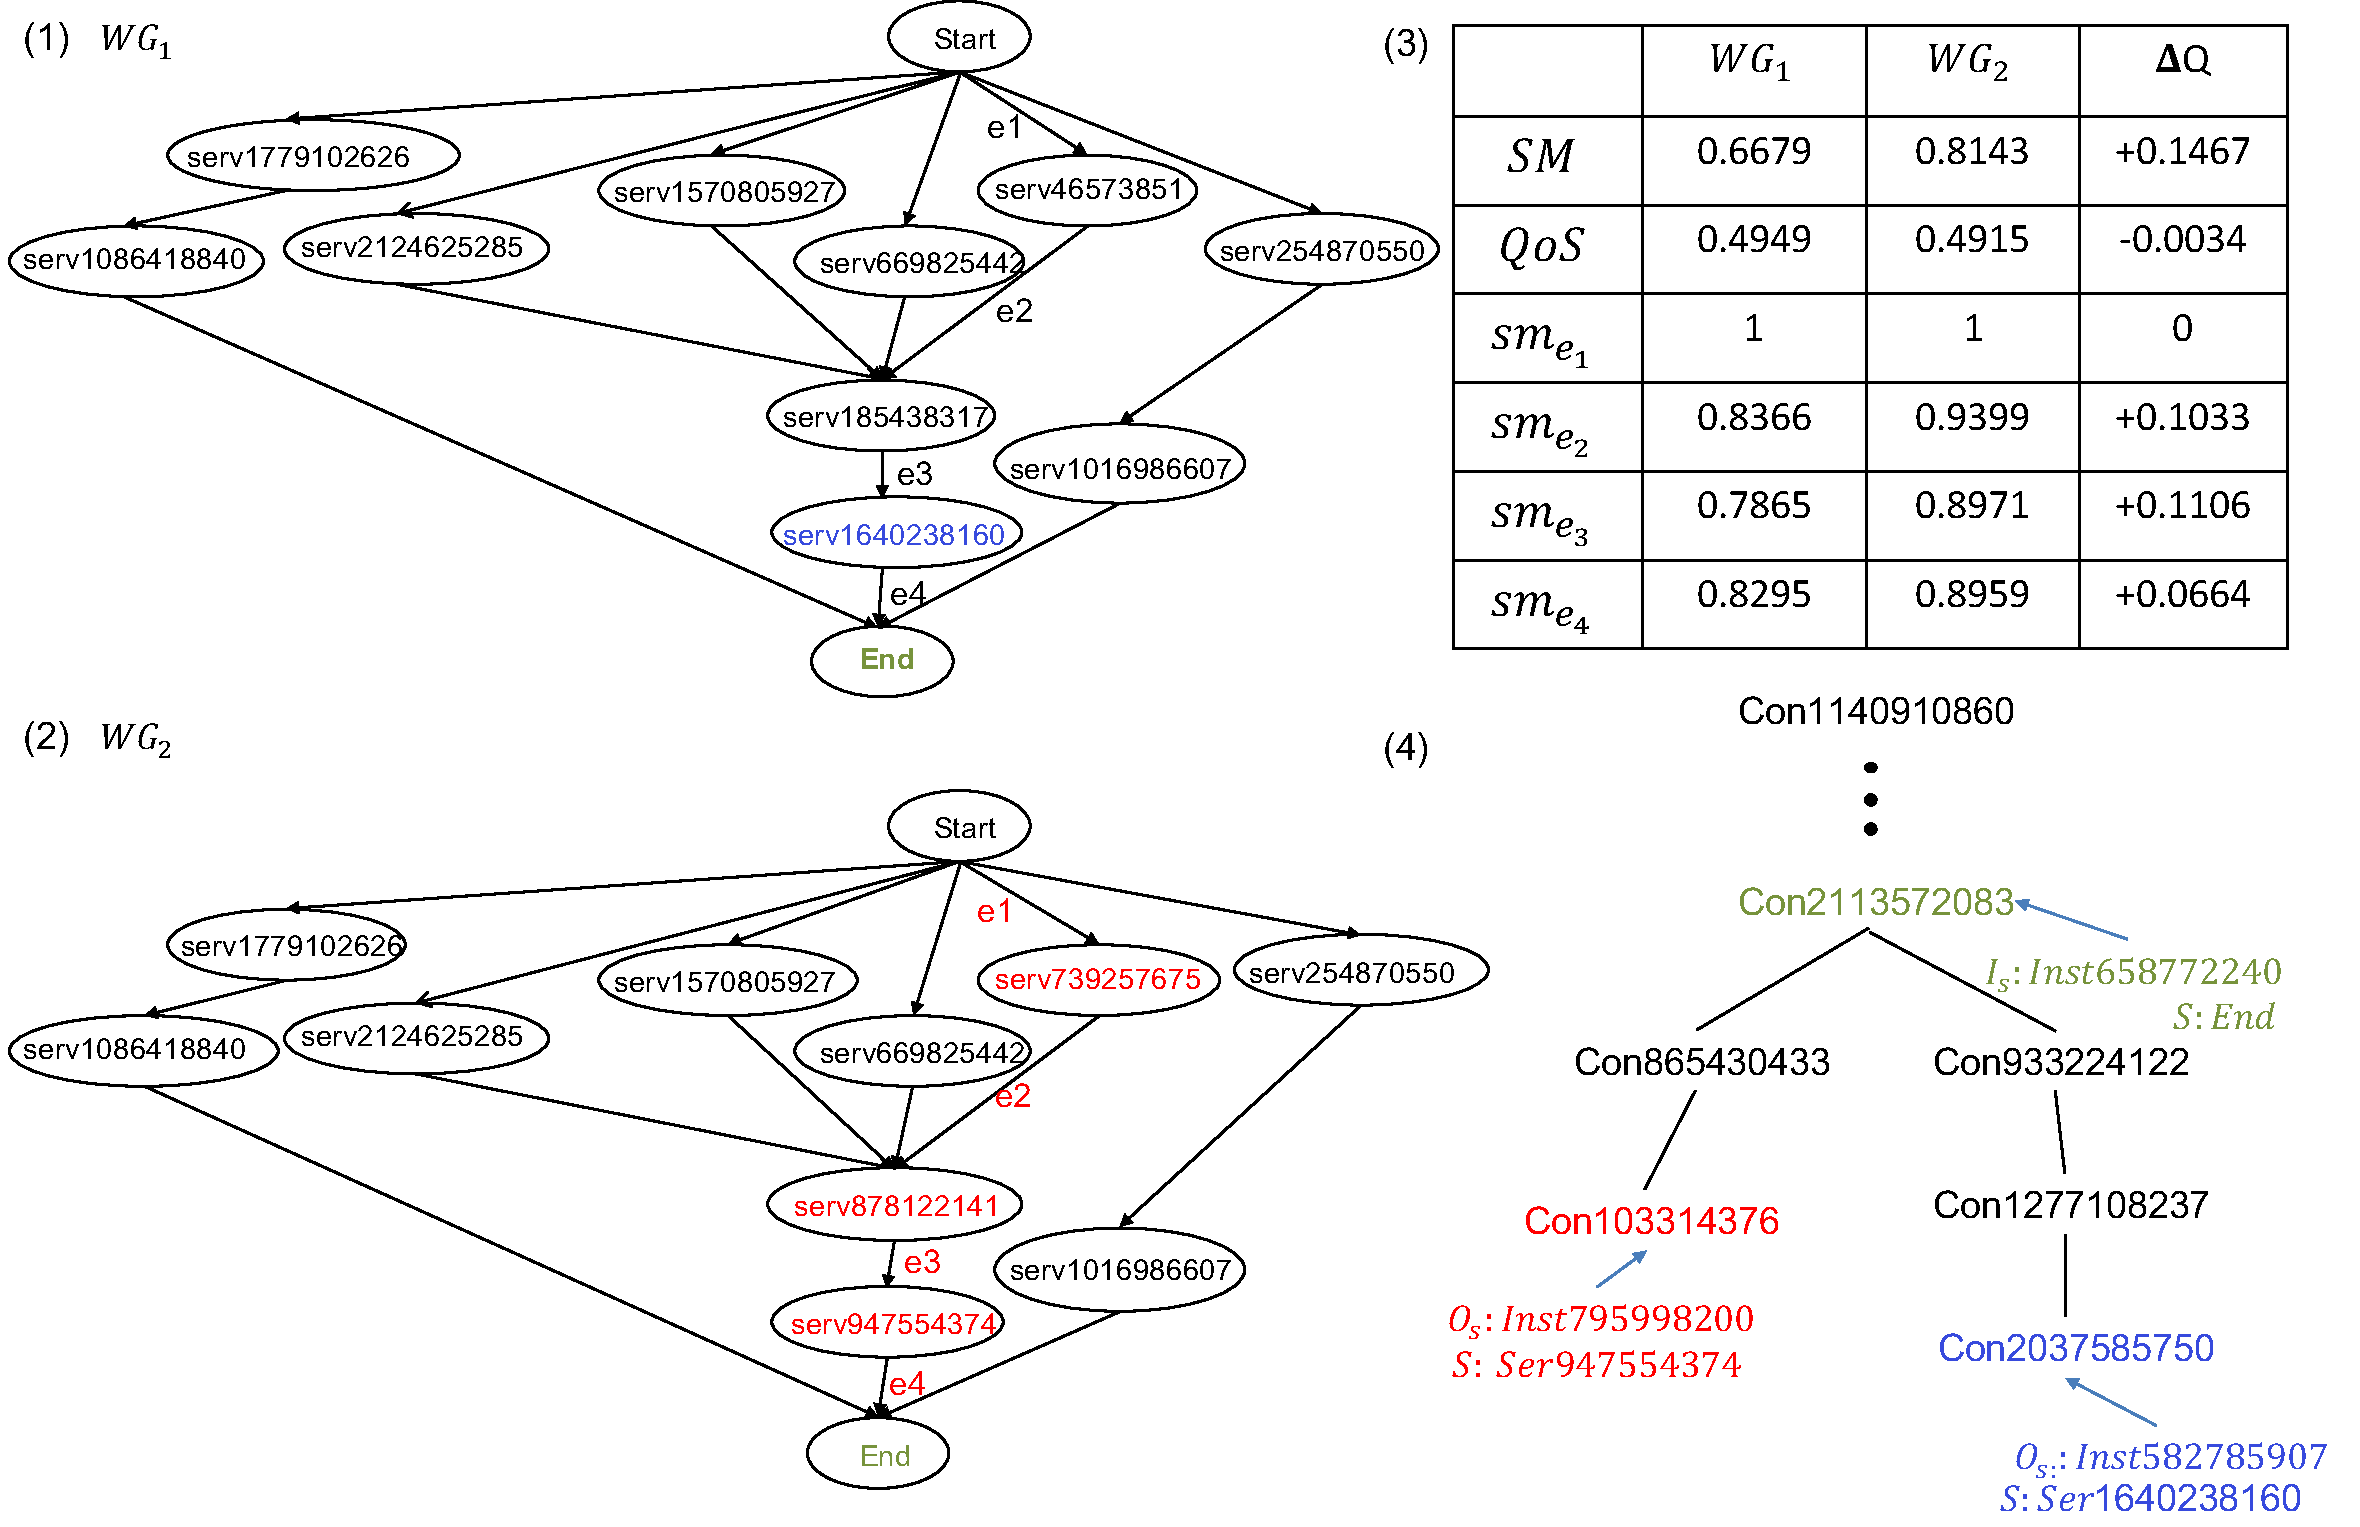
\includegraphics[scale=.29]{comparisontest.pdf}}}
 \caption{An example of comparision to optimal solutions using Task 3 for QoS evaluation model and comprehensive quality evluation model.}
 \label{comparisontest}
\end{figure}


\section{Conclusion}\label{conclusion}
This work introduces a comprehensive evaluation model for considering semantic matchmaking quality and QoS simultaneously. We proposed a PSO-based service composition approach utilising our proposed quality mode that can achieve a desirable trade-off of both quality aspects. In addtion, we compare one recent GP-approach with our PSO-based method to show our performance that results in finding more optimised solutions. Future works can investigate multi-objective EC techniques to produce a set of composition solutions for the situations when the quality preference is not known.


\bibliographystyle{splncs03}
\bibliography{IEEEexample}

\end{document}